\chapter{Results} \label{chap:experiments}

\section{Data}
Two datasets were used in the experiments, our collected dataset HuPBA-AgeGuess and the classic benchmark database FG-NET.


\textbf{FG-NET} consists of 1002 frontal face images of 82 different individuals. The image quality varies a lot in the dataset since there are images in grey scale and RGB. The face position is frontal and under similar illumination conditions. The dataset also contain 68 facial landmarks for each face image.

\begin{figure}[!h]
	\centering
	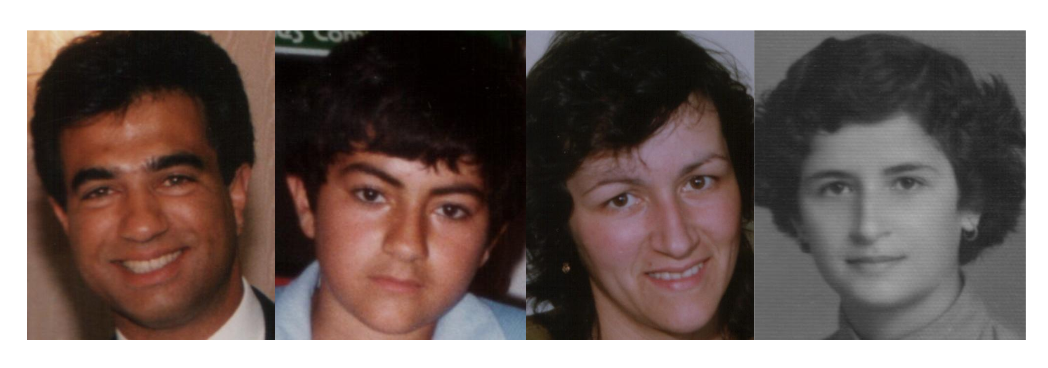
\includegraphics[width=\textwidth]{figures/FGNET_sample}
	\caption{FG-NET image samples.}
	\label{fig:imgSample1}
\end{figure}

\textbf{HuPBA-AgeGuess} dataset (\ref{fig:imgSample2}) used in this project is a subset of the 4865 images filtered out by a minimum number of votes per image. This subset contains 3398 face images. The images are captured in the wild so the faces position vary up to $\pm90º$ and the illumination is also different in every picture.

\begin{figure}[!h]
	\centering
	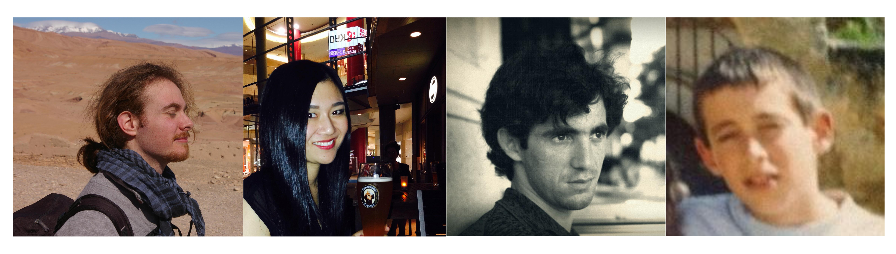
\includegraphics[width=\textwidth]{figures/HuPBA_sample}
	\caption{HuPBA-AgeGuess image samples.}
	\label{fig:imgSample2}
\end{figure}

\section{Methods and Parameters}
\section{Experimental Settings}

\section{Experiments}

\begin{figure}[!h]
	\centering
	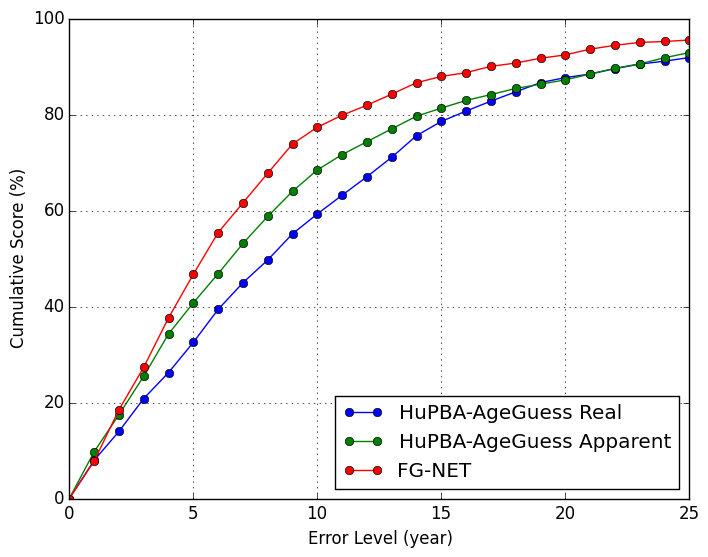
\includegraphics[width=\textwidth]{figures/cum_score}
	\caption{Cummulative Score }
	\label{fig:cumS}
\end{figure}